\begin{center}
  \scalebox{1.3}{
    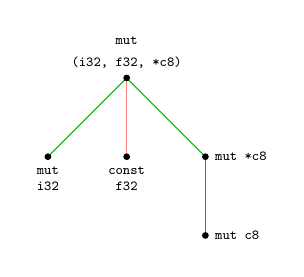
\begin{tikzpicture}

      \draw[-, black!30!green] (0,0) -- (-1,-1);
      \draw[-, red!50] (0,0) -- (0,-1);
      \draw[-, black!30!green] (0,0) -- (1,-1);
      \draw[-, black!30!green] (1,-1) -- (1,-2);

      \filldraw (0, 0.3) node[align=center, above] {\texttt{\tiny{mut}}};
      \filldraw (0, 0) circle (1pt) node[align=center, above] {\texttt{\tiny{(i32, f32, *c8)}}};
      \filldraw (-1,-1) circle (1pt) node[align=center, below]{\texttt{\tiny{mut}}};
      \filldraw (-1,-1.2) node[align=center, below]{\texttt{\tiny{i32}}};
      \filldraw (0,-1) circle (1pt) node[align=center, below]{\texttt{\tiny{const}}};
      \filldraw (0,-1.2) node[align=center, below]{\texttt{\tiny{f32}}};
      \filldraw (1,-1) circle (1pt) node[align=center, right]{\texttt{\tiny{mut *c8}}};
      \filldraw (1,-2) circle (1pt) node[align=center, right]{\texttt{\tiny{mut c8}}};


    \end{tikzpicture}
  }
  \captionof{figure}{\label{fig:tuple_mutability} Example of tuple mutability}
\end{center}
